\section{Ejercicio 1}\label{sec:ejercicio1}

\begin{frame}{Oscilador Amortiguado}
    \begin{multicols}{2}
        % First column with the text
        {
        \begin{itemize}
            \item Masa de la partícula - $m = 70\ \text{kg}$
            \item Tiempo de simulación - $t_f = 5\ \text{s}$
            \item Constante elástica - $k = 10000\ \text{kg/s}^2$
            \item Viscosidad - $\gamma = 100\ \text{kg/s}$
            \item Amplitud inicial - $A = 1\ \text{m}$
        \end{itemize}
        }
        {
        % Second column with the "animation" image
        \begin{figure}[H]
            \centering
            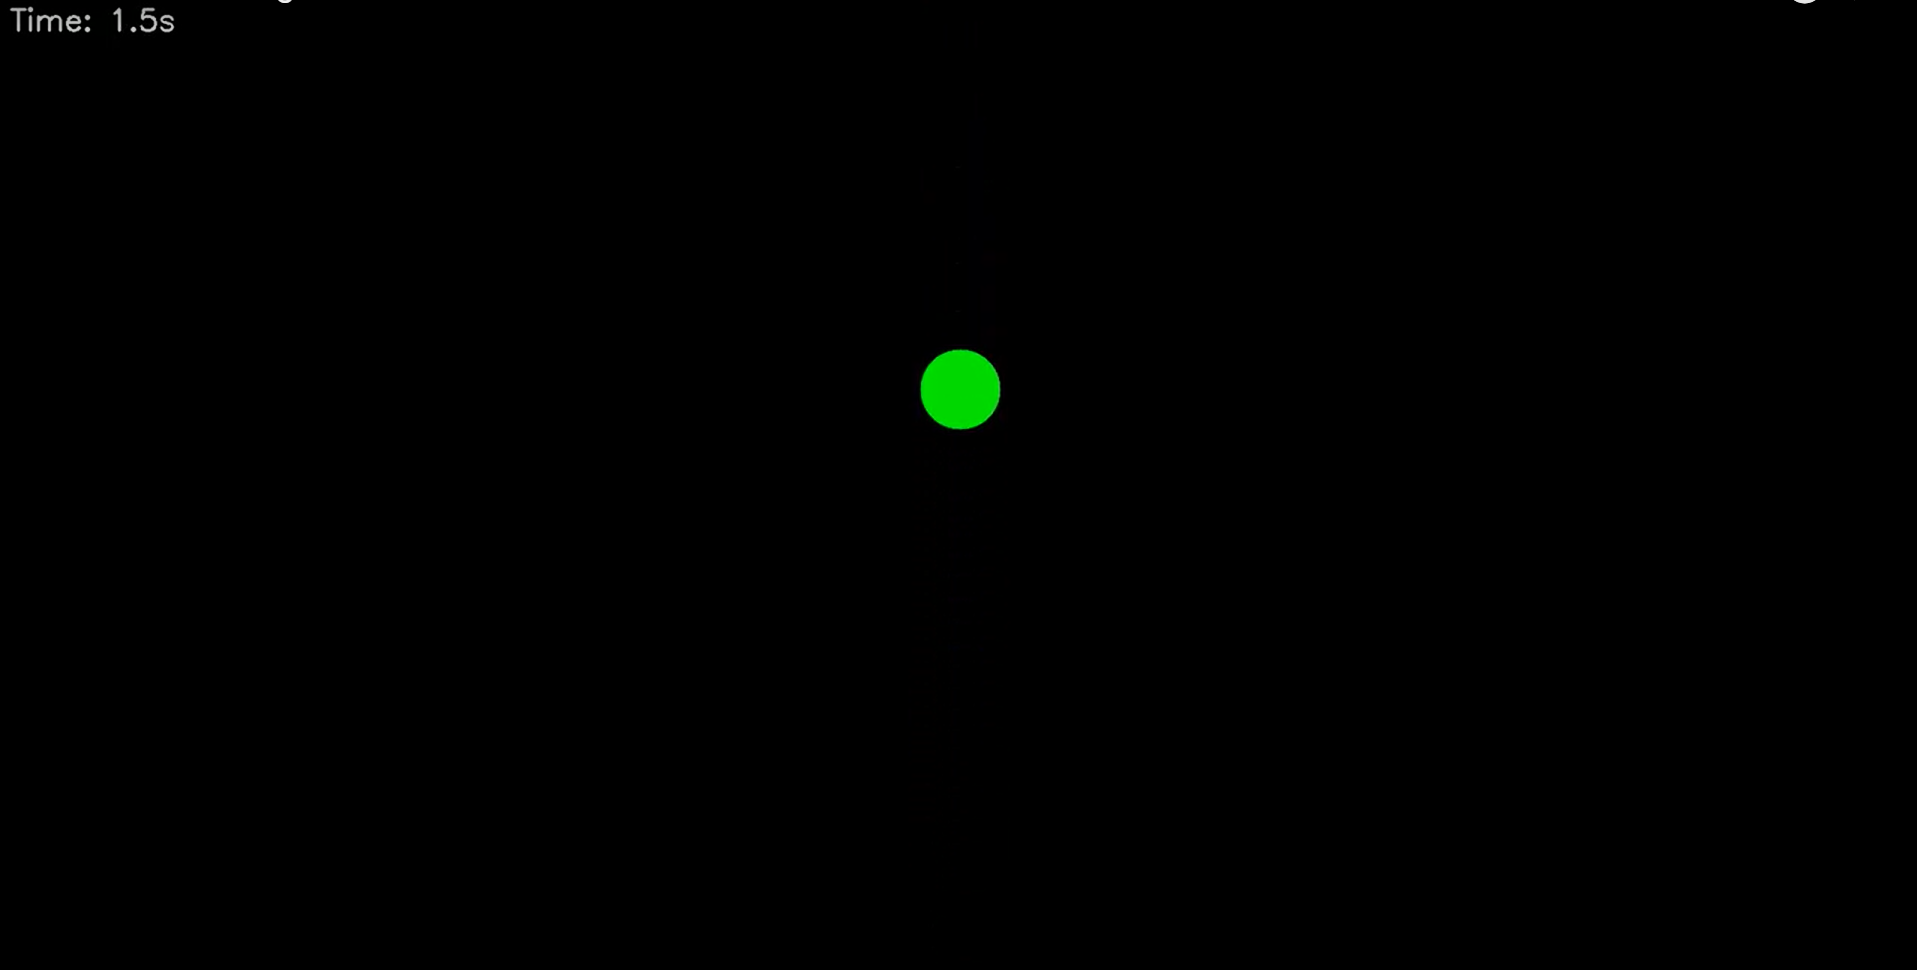
\includegraphics[width=1\linewidth]{pic/00-ejercicio1/thumbnail}\\
            \captionsetup{font={scriptsize}}
            \captionsetup{labelformat=empty}
            \caption{\href{https://www.youtube.com/watch?v=X2C-ouZ1_7g}{https://www.youtube.com/watch?v=X2C-ouZ1\_7g}}
            \label{fig:oscilador_amortiguado_animation}
        \end{figure}
        }
    \end{multicols}
\end{frame}


\begin{frame}{Oscilador Amortiguado}
    \begin{figure}[htbp]
        \centering
        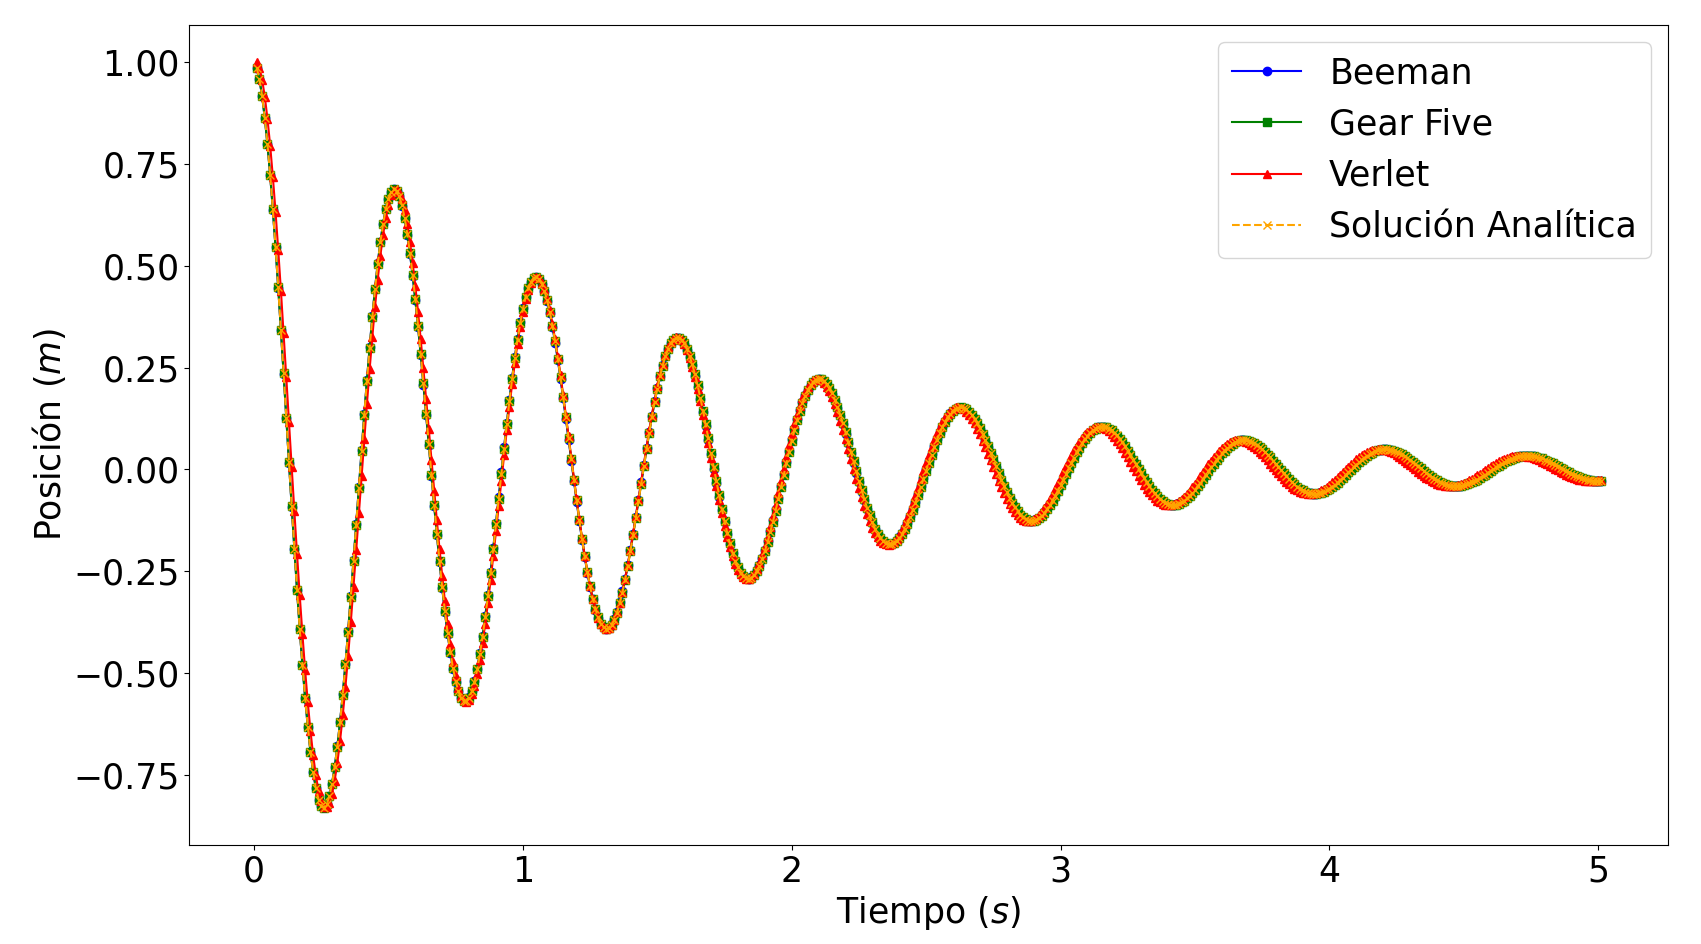
\includegraphics[width=0.9\linewidth]{pic/00-ejercicio1/todos}
        \label{fig:osc_amortiguado}
    \end{figure}
\end{frame}

\begin{frame}{Oscilador Amortiguado}
    \begin{figure}[htbp]
        \centering
        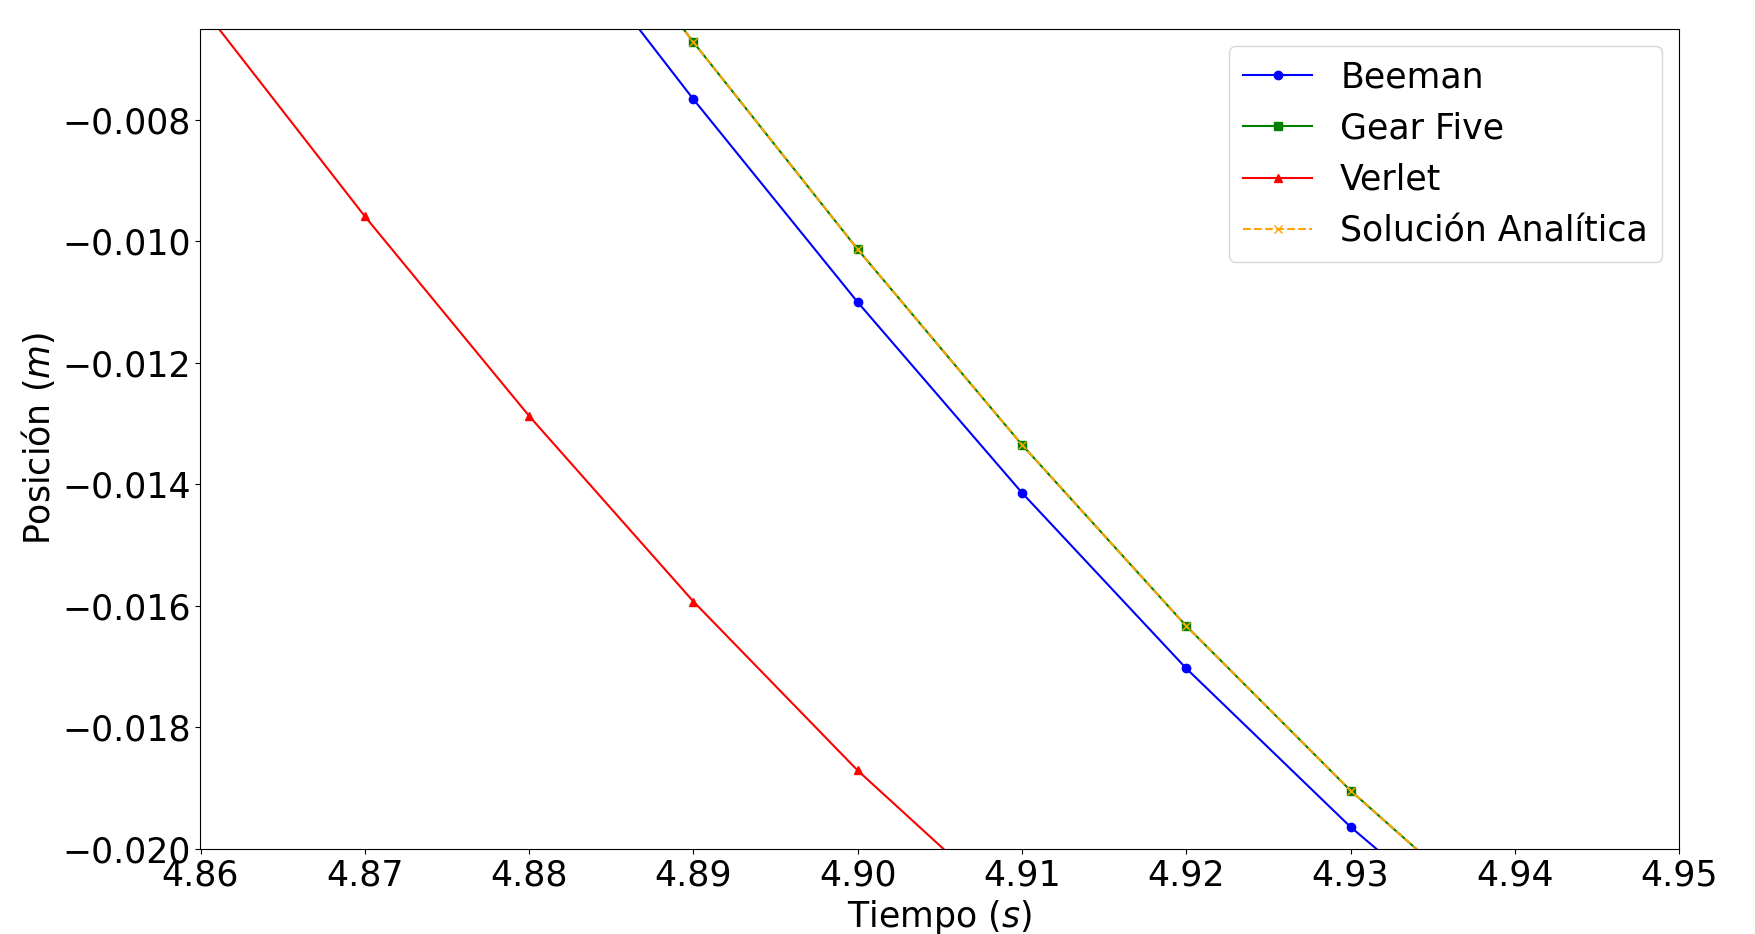
\includegraphics[width=0.9\linewidth]{pic/00-ejercicio1/zoom}
        \label{fig:osciladore-zoom}
    \end{figure}
\end{frame}

\begin{frame}{Oscilador Amortiguado}
    \begin{figure}[H]
        \centering
        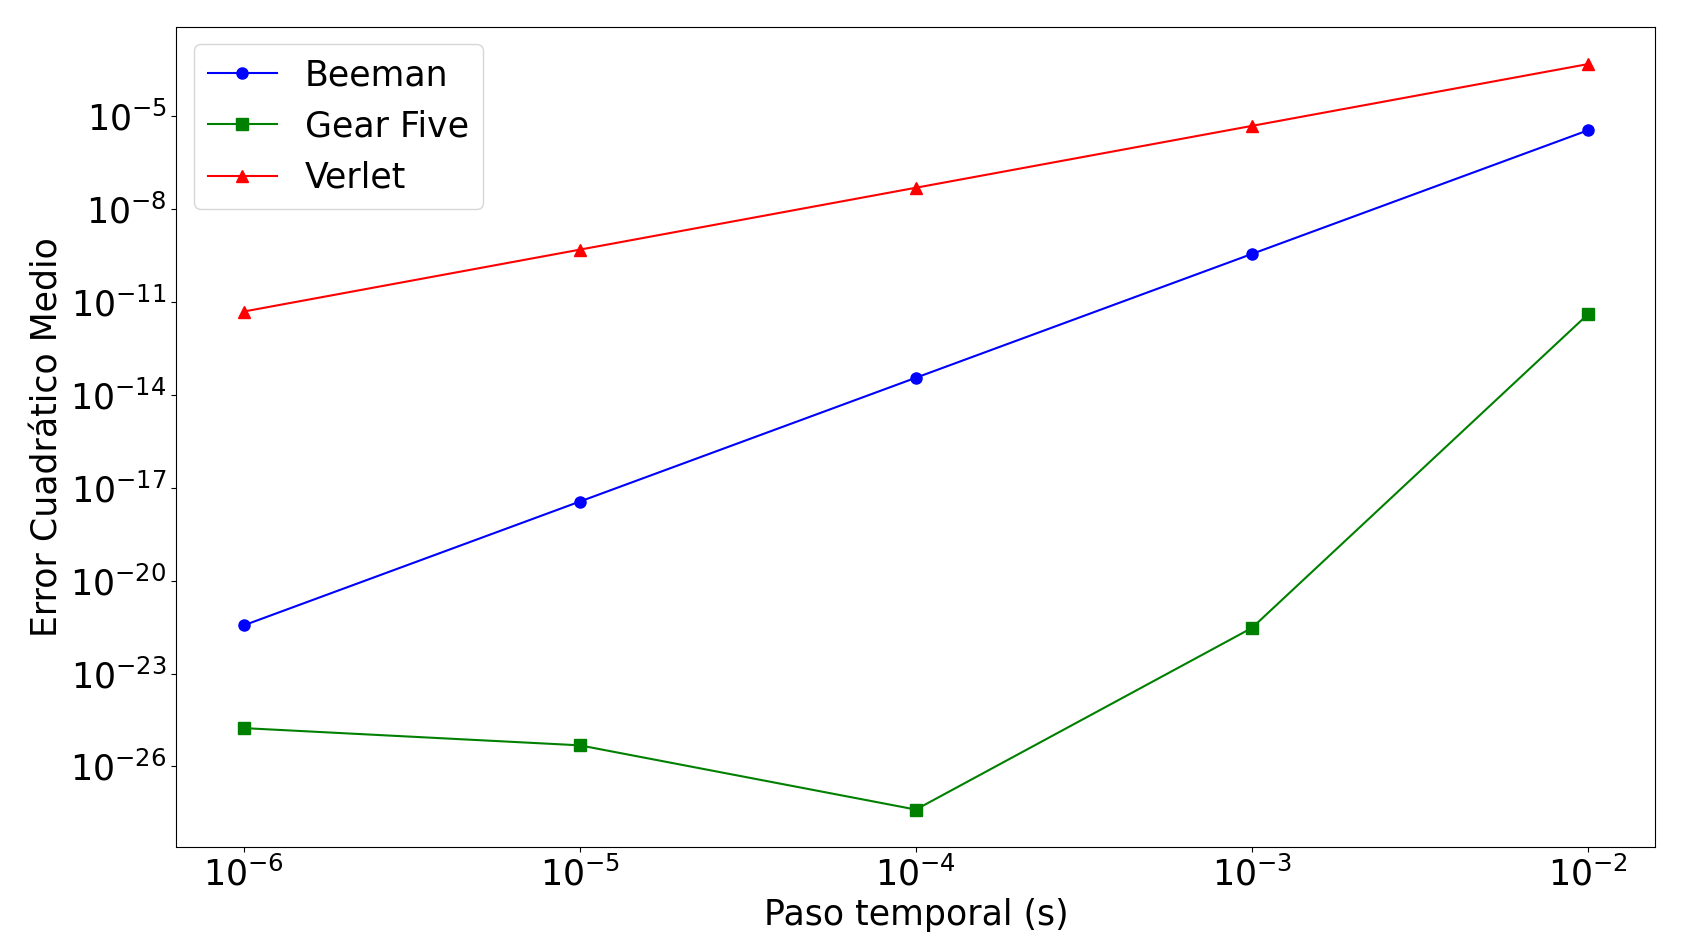
\includegraphics[width=0.9\linewidth]{pic/00-ejercicio1/ECMs}
        \label{fig:osciladore-ECM}
    \end{figure}
\end{frame}

